Last updated: 19-10-2020 18:15

\documentclass[11pt]{amsart}
\usepackage{geometry}                % See geometry.pdf to learn the layout options
	\geometry{a4paper}  

\usepackage{enumitem}
\usepackage{graphicx}
\usepackage{subcaption}
\usepackage{amsmath}
\usepackage{amssymb}
\usepackage{epstopdf}
\usepackage{setspace}
\usepackage{listings}

\lstdefinestyle{myListingStyle} 
    {
        basicstyle = \small\ttfamily,
        breaklines = true,
    }

\graphicspath{ {./assets/} }

\DeclareGraphicsRule{.tif}{png}{.png}{`convert #1 `dirname #1`/`basename #1 .tif`.png}
%\setkomafont{title}{\normalfont\scshape}
%\addtokomafont{disposition}{\rmfamily}

%\newcommand{\subtitle}{A review of previous work and avenues for future research}
    
\title{Percolation and the Firefighter Problem}
\author{Ethan Kelly}
%\author{Supervisor: Jessica Enright}

\newcommand{\Addresses}{{% additional brackets for segregating \footnotesize
  \bigskip
  \footnotesize
  \textsc{Ethan Kelly} \par\nopagebreak
  	\hspace{\parindent}\textit{Email:~}\texttt{E.Kelly.1@research.gla.ac.uk}\par\nopagebreak
	\vspace{1mm}
  \textsc{Supervisor: Jessica Enright}\par\nopagebreak
  	\hspace{\parindent}\textit{Email:~}\texttt{Jessica.Enright@glasgow.ac.uk}\par\nopagebreak
	\vspace{1mm}
	\begin{flushright}
  \textsc{Department of Computing Science\\Sir Alwyn Williams Building\\University of Glasgow\\G12 8QN}
  \end{flushright}
}}

%%%%%%%%%%%%%%%%%%%%%%%%%%%%%%%%%%%%%%%%%%%%%%%%%%

\begin{document}
\maketitle
\Addresses
\section{Introduction}
\label{sec:intro}

The Firefighter Problem was first discussed by Hartnell in 1995 \cite{hartnell95} and models an outbreak of fire with a firefighter strategically blocking its path. We will discuss this original formulation of the problem and explain how it can be used in applications from the spread of disease to the spread of viral content on social media.\\

The other topic we will address is Percolation Theory, and how it proves very promising in answering questions about the Firefighter Problem. We will outline the original conception and the context it was considered and explain how a slight variant will prove far more useful for our purposes in considering the Firefighter Problem.

%%%%%%%%%%%%%%%%%%%%%%%%%%%%%%%%%%%%%%%%%%%%%%%%%%

\section{Background}

\subsection{Firefighter}
\label{sec:fire}

The Firefighter Problem, which we refer to as simply {\scshape Firefighter}, is the focus and motivation of our discussion; we, in particular, hope to show that Percolation can provide many answers to questions asked about {\scshape Firefighter}. We first formalise {\scshape Firefighter} as follows: at $t=0$, fire breaks out at some vertex $v_0$ of graph $G$. The firefighter then `protects' another vertex\footnote{\,This has been extended to $n$ vertices in some research, but here we wish to illustrate for simplicity the original form of the problem.} of $G$. A protected vertex is protected for the remainder of the game; it is inflammable \textit{ad infinitum.} Similarly, a vertex that has been on fire is `burnt' for the rest of the game and cannot ignite again. The fire spreads to any immediate neighbouring vertices that are neither protected nor burnt. Then, the firefighter may protect another vertex, the fire spreads again and so on.\footnote{\,It may be tempting to put the firefighting move and the fire spread into two distinct time steps, $t$ and $t+1$ - this is beneficial in some applications (such as two player versions of {\scshape Firefighter}) but in general will make computation more time consuming.} The following is a decision formulation given by Finbow and MacGillivray for {\scshape Firefighter} on a tree \cite{finbow09}:


{\scshape Firefighter}\\ \indent
{\scshape Instance:} A rooted graph $(G,r)$ and an integer $k\geq 1$.\\ \indent
{\scshape Question:} Is there a finite sequence $d_1, d_2,\dots d_t$ of vertices of the graph $G$ such that:
	\begin{enumerate}[label=\roman*]
		\item $d_i$ {is neither burned nor defended at time} $i$,
		\item {At time} $t$, no undefended vertex is adjacent to a burning vertex, and
		\item {At least} $k$ {vertices are saved at the end of time} $t$?
	\end{enumerate}

Common questions to ask in {\scshape Firefighter} include: how do we minimise the number of vertices that will be burnt? In a given class of trees, what is the average number of burnt vertices? Is the problem NP-complete?\\

There are many natural contextualisations of {\scshape Firefighter} - for instance, let each vertex be an individual and let the edges between them represent social contact. This is a simple model for disease infection. If instead we think of these edges representing virtual contact between individuals on social media, we have a model for the spread of viral internet memes \cite{obrien19}.

%%%%%%%%%%%%%%%%

\subsection{Percolation Theory}
\label{sec:perc}

Widely known and used in physics, statistics and mathematics, Percolation theory involves modelling scenarios as $n$-dimensional graphs, so application to {\scshape Firefighter} is not entirely unexpected. The edges between vertices in the graph can be either `open' or `closed' with probability $p$ and $1-p$ respectively. We can think of percolation problems as liquid being poured onto a porous material and whether there is a path from hole to hole along open paths through the material. Note that removing more and more edges mov†es us towards a critical point at which removing further edges would cause the graph to fall apart into smaller clusters of vertices and edges that have no access to each other \cite{grimmett99}. This is known as `bond' percolation, as edges correspond to bonds in many of its applications.\\
\begin{figure}[ht]
	\centering
		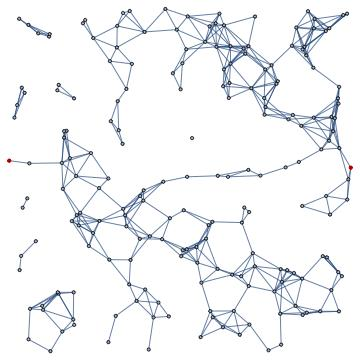
\includegraphics[width=0.45\linewidth]{percolated-graph.jpg}
	\caption{A graph at its percolation threshold \cite{mathematica17} (Mathematica code in in Appendix \ref{apx:mathematica}).}
	\label{fig:percolated-graph}
\end{figure}
Several authors have suggested percolation as a possible approach to {\scshape Firefighter} \cite{finbow09}. In this context, we could determine the critical point to see how we might contain the fire to a smaller cluster that cannot spread to the wider graph. For {\scshape Firefighter}, site percolation is more applicable: rather than considering open or closed \emph{edges} (`bonds') between vertices as in bond percolation, we consider each \emph{vertex} (`site') as being `occupied' or `unoccupied' with probability $p$ and $1-p$ respectively.\\

Formally, we consider a point lattice $\mathbb{L}$ and denote the open cluster as $C(x)\text{,~where~}x\in\mathbb{L}$ is the local origin of the cluster. This cluster $C(x)$ is defined as the set of all vertices that can be reached from open paths beginning at the nucleation site, $x$. Then, we are particularly interested in the \emph{percolation probability}:
$$
\theta(p) = \mathbb{P}_p(\,|C(0)|=\infty\,),
$$
and the \emph{critical probability} (or \emph{percolation threshold}):
$$
p_c = \sup\{\,p \mid \theta(p)=0\,\}.
$$
Here, $\mathbb{P}_p$ is the product measure given by:
$$
\displaystyle \mathbb{P}_p=\prod_{v\in\mathbb{L}^d}\mu_v
$$
where $\mu_v$ is the \emph{Bernoulli measure}, which returns $p$ when $v$ is open and $1-p$ when $v$ is closed \cite[p. 28]{klenke14}. Analytically, others have shown that in the case of a two-dimensional regular point lattice, the critical probability is $p_c=1/2$ \cite{kersten80}.

%%%%%%%%%%

\section{Potential Uses of Percolation in The Firefighter Problem}

We have identified three main avenues that may be pursued in {\scshape Firefighter} using Percolation: the firefighter may use percolation in order to defend the graph, the fire might spread with percolation probability $p$ or we might use percolation on the graph to form a more useful model (i.e. one that can more accurately represent an irregular population density). The former might be used when the firefighter can save more than one vertex at each turn; the latter may be more useful when modelling disease spread.
\begin{figure}[ht]
	\centering
		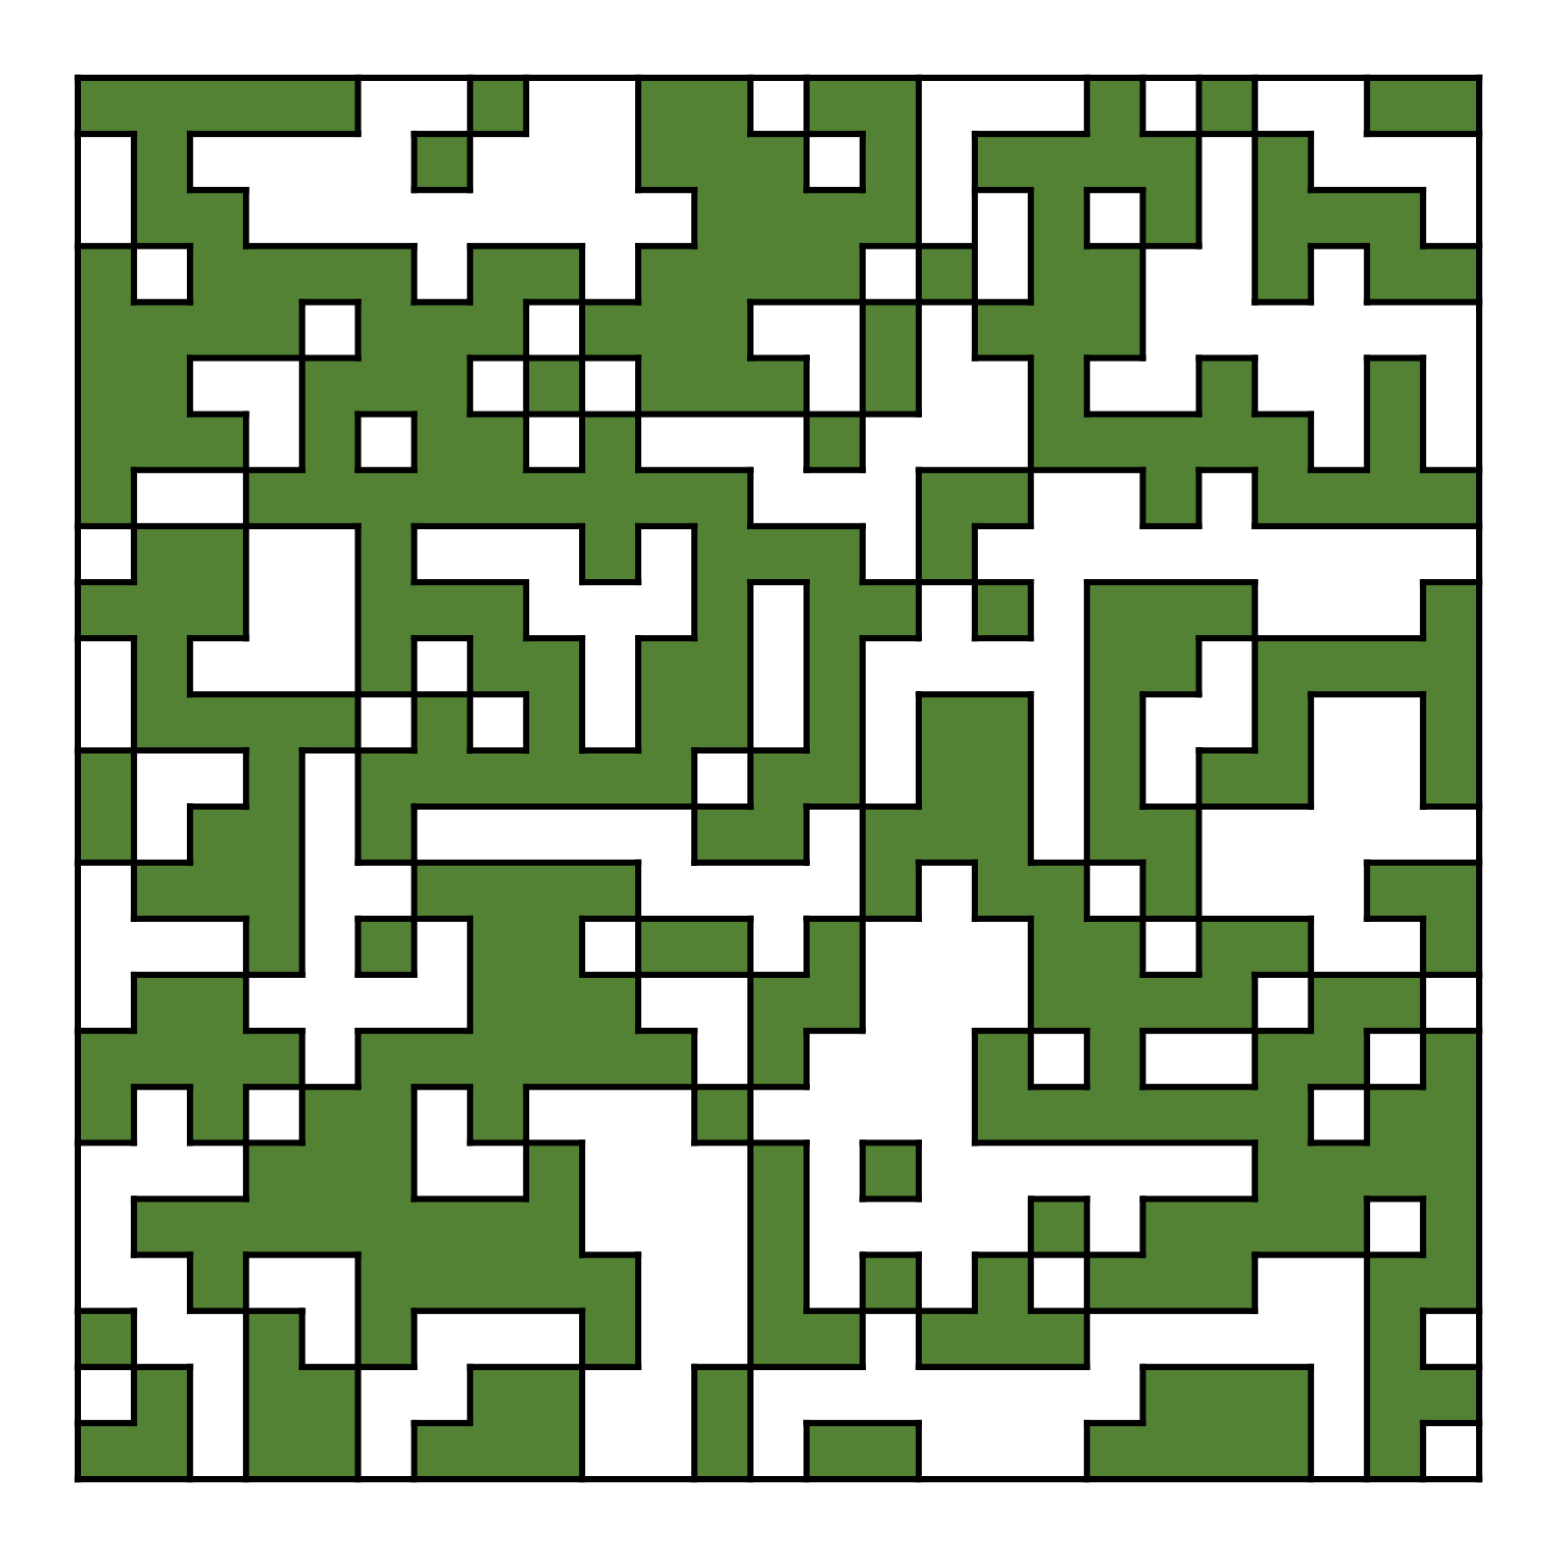
\includegraphics[width=0.3\linewidth]{firebreak/25x25/25x25}
	\caption{A regular $(25\times25)$ graph, percolated with probability $p=2/3$.}
	\label{fig:largeperc}
\end{figure}

%%%%%%%%%%

\subsection{Better than random}
One potential use for the firefighter using percolation as a method of defence would be as a baseline test: in most scenarios, a method for obtaining defence strategies should be at least as effective as a random defence sequence. We could find such a random sequence using percolation for comparison purposes. Consider a sequence of vertices in graph $G$, written as $d_1, d_2,\dots, d_t$. An optimal defence sequence could be found using integer programming as provided by Finbow and MacGillivray \cite{finbow09}:
\begin{equation*}
	\begin{array}{ll@{}ll}
\text{Maximise}  & \displaystyle \sum\limits_{v\in V(G)} d_v w(v) &\text{~for each level~} i\\
\text{subject to}& d_v + \displaystyle\sum\limits_{\text{level}(v)=i} d_v \leq 1  &\text{~for each level~} i\\
				 & d_v + \displaystyle\sum\limits_{u\succ v}  d_u \leq 1  &\text{~for every outer vertex~} v \text{~of~} T,\\
                 &d_{v} \in \{0,1\}. &
	\end{array}
\end{equation*}
where $u\succ v$ indicates that $u$ is an ancestor of $v$. The optimal strategies provided for different classes and densities of graphs here will provide an upper bound (which may indeed be impossible to attain in some cases) for success of a given strategy. We can find a lower bound using percolation, and so we have a range of success values as a starting point: if some strategy is better than random percolation, then it is worth considering, but below the particular expected optimal solution from integer programming and we can improve or find a better strategy.\\

We conjecture that, at the lowest graph densities, the random strategy will be very close to the optimal strategy and thus finding an improvement is at once difficult and lacking in great utility. At the very highest graph densities, while random strategies will have a very low expected best-case scenario, as will most strategies as the constraint on the firefighter that they have only one vertex to save per turn does not go as far when vertices are much better connected. Thus, finding improvements on random will again not prove very useful as random and best-case scenarios serve to show us that there is a small range of possible, not good outcomes.

\subsection{Reproduction rate}
We now focus our attention on the fire spread being determined by percolation (rather than the firefighter's defence sequence). Diseases, when there is a large enough sample size, have a basic reproduction rate associated with them, denoted $R_0$: for instance, measles has a basic reproduction rate $12\leq R_0 \leq 18$ \cite{fiona17} and the Influenza strain responsible for the 1918 pandemic has a basic reproduction rate of $1.4 \leq R_0 \leq 2.8$ \cite{ferguson06}. These values correspond to a basic expectation \\

Where we wish to consider vertices as individuals and edges as the connections between them, percolation may give us a more useful model for disease spread when we do not assume the population is well mixed and instead introduce probability functions to correspond to the likelihood one vertex is connected to another.\\

\subsection{Irregular population density}
A great deal of the literature surrounding {\scshape Firefighter} assumes a regular graph - that is, in the context of disease we assume a well-mixed population where everyone has equal probability of coming into contact with their neighbours. Of course, this is a significant simplification of reality: some individuals are very well connected and have lots of contact with others, whereas some people have significantly less contact with others. In the context of a forest fire, the density of a forest is irregular and there is a probability in the unit interval that fire can spread between two trees depending on their proximity (among other factors): an example of this can be seen in figure \ref{fig:largeperc}. Thus, percolation on regular grids to more closely resemble populations or forest density could lead to far more useful and realistic modelling results.\\

\begin{figure}[!ht] 
  \begin{subfigure}{0.4\linewidth}
    \centering
    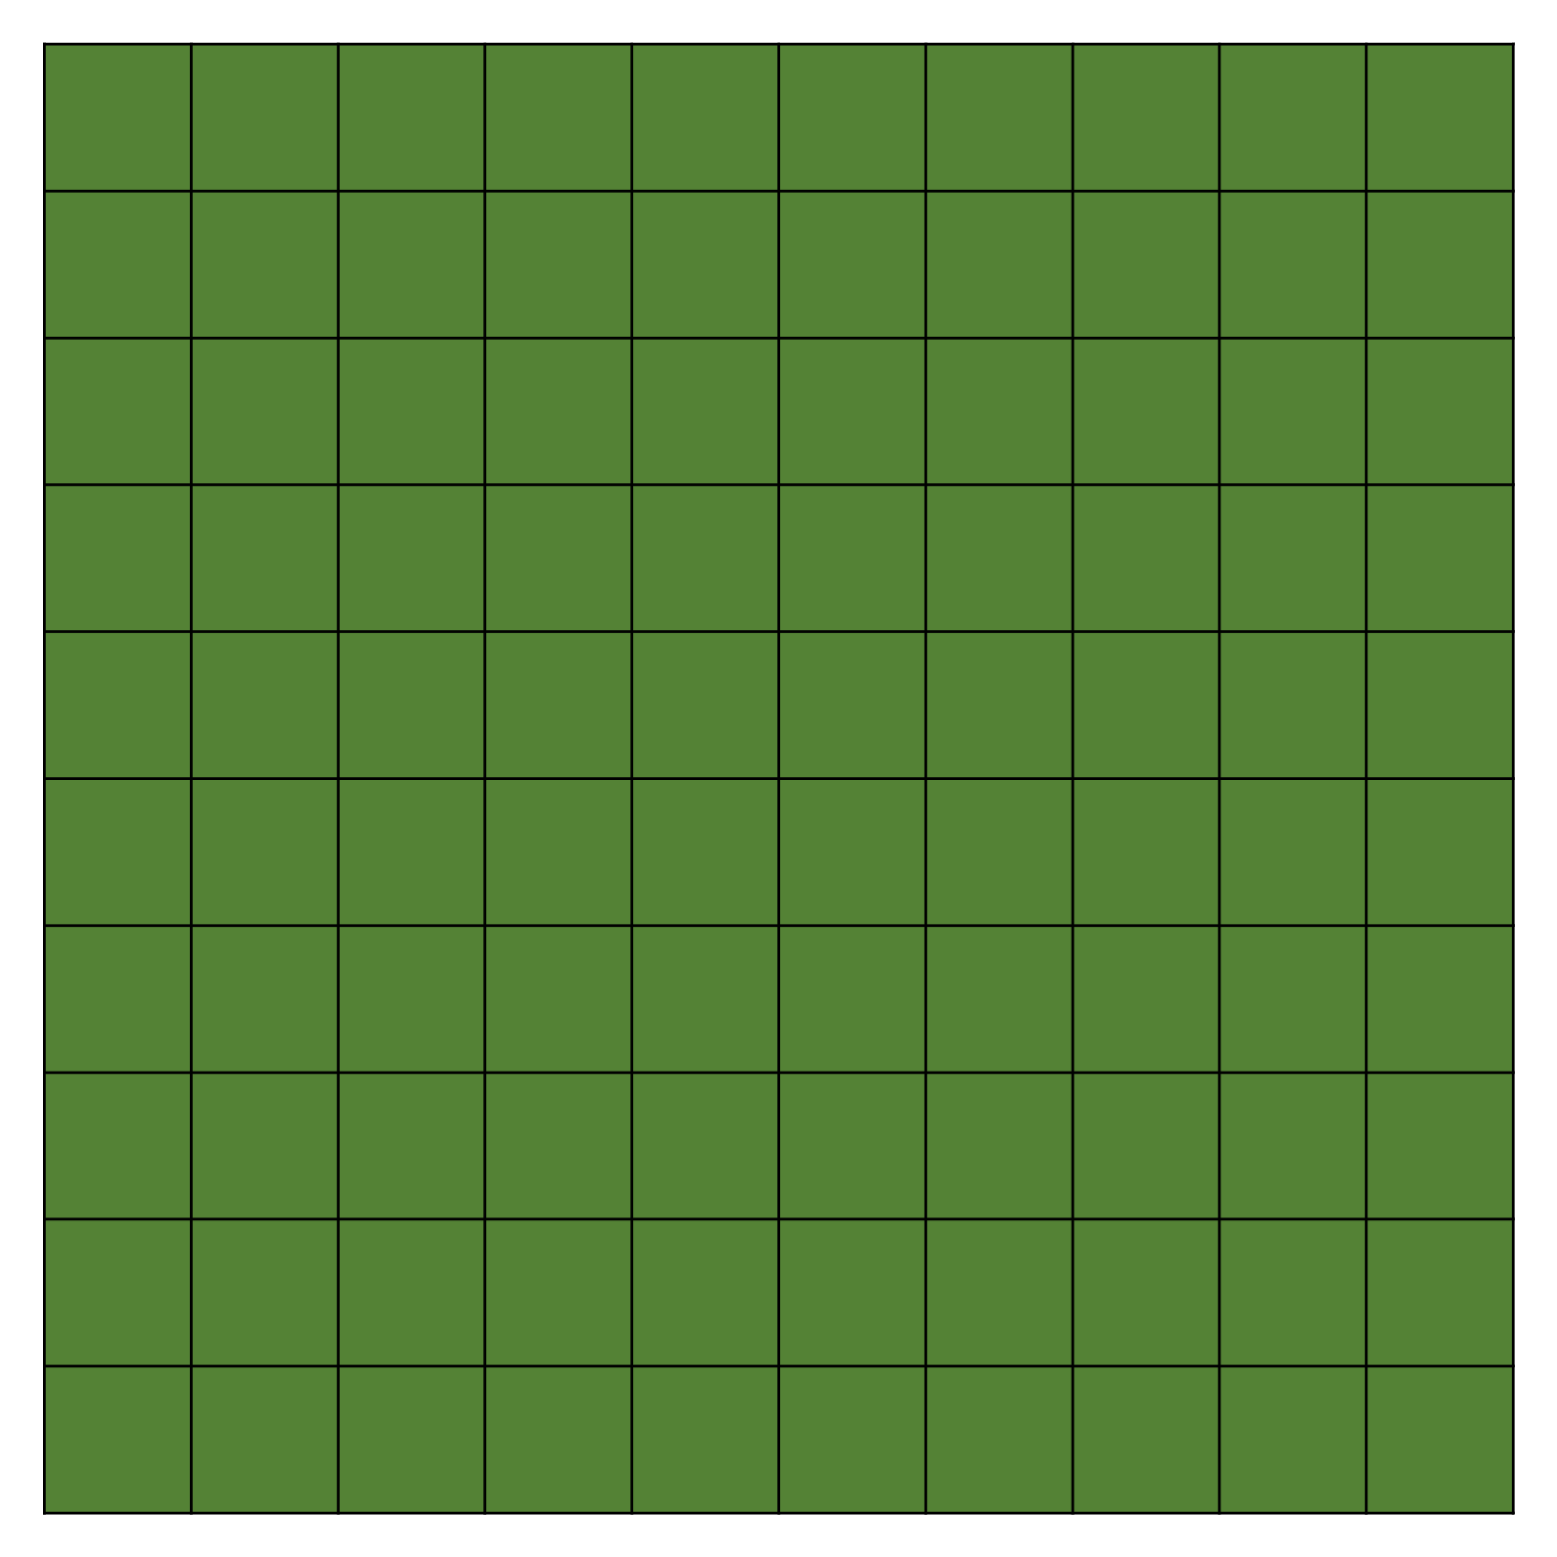
\includegraphics[width=0.4\linewidth]{firebreak/original} 
    \caption{Initial regular graph} 
    \label{fig:original} 
    \vspace{4ex}
  \end{subfigure}%% 
  \begin{subfigure}{0.4\linewidth}
    \centering
    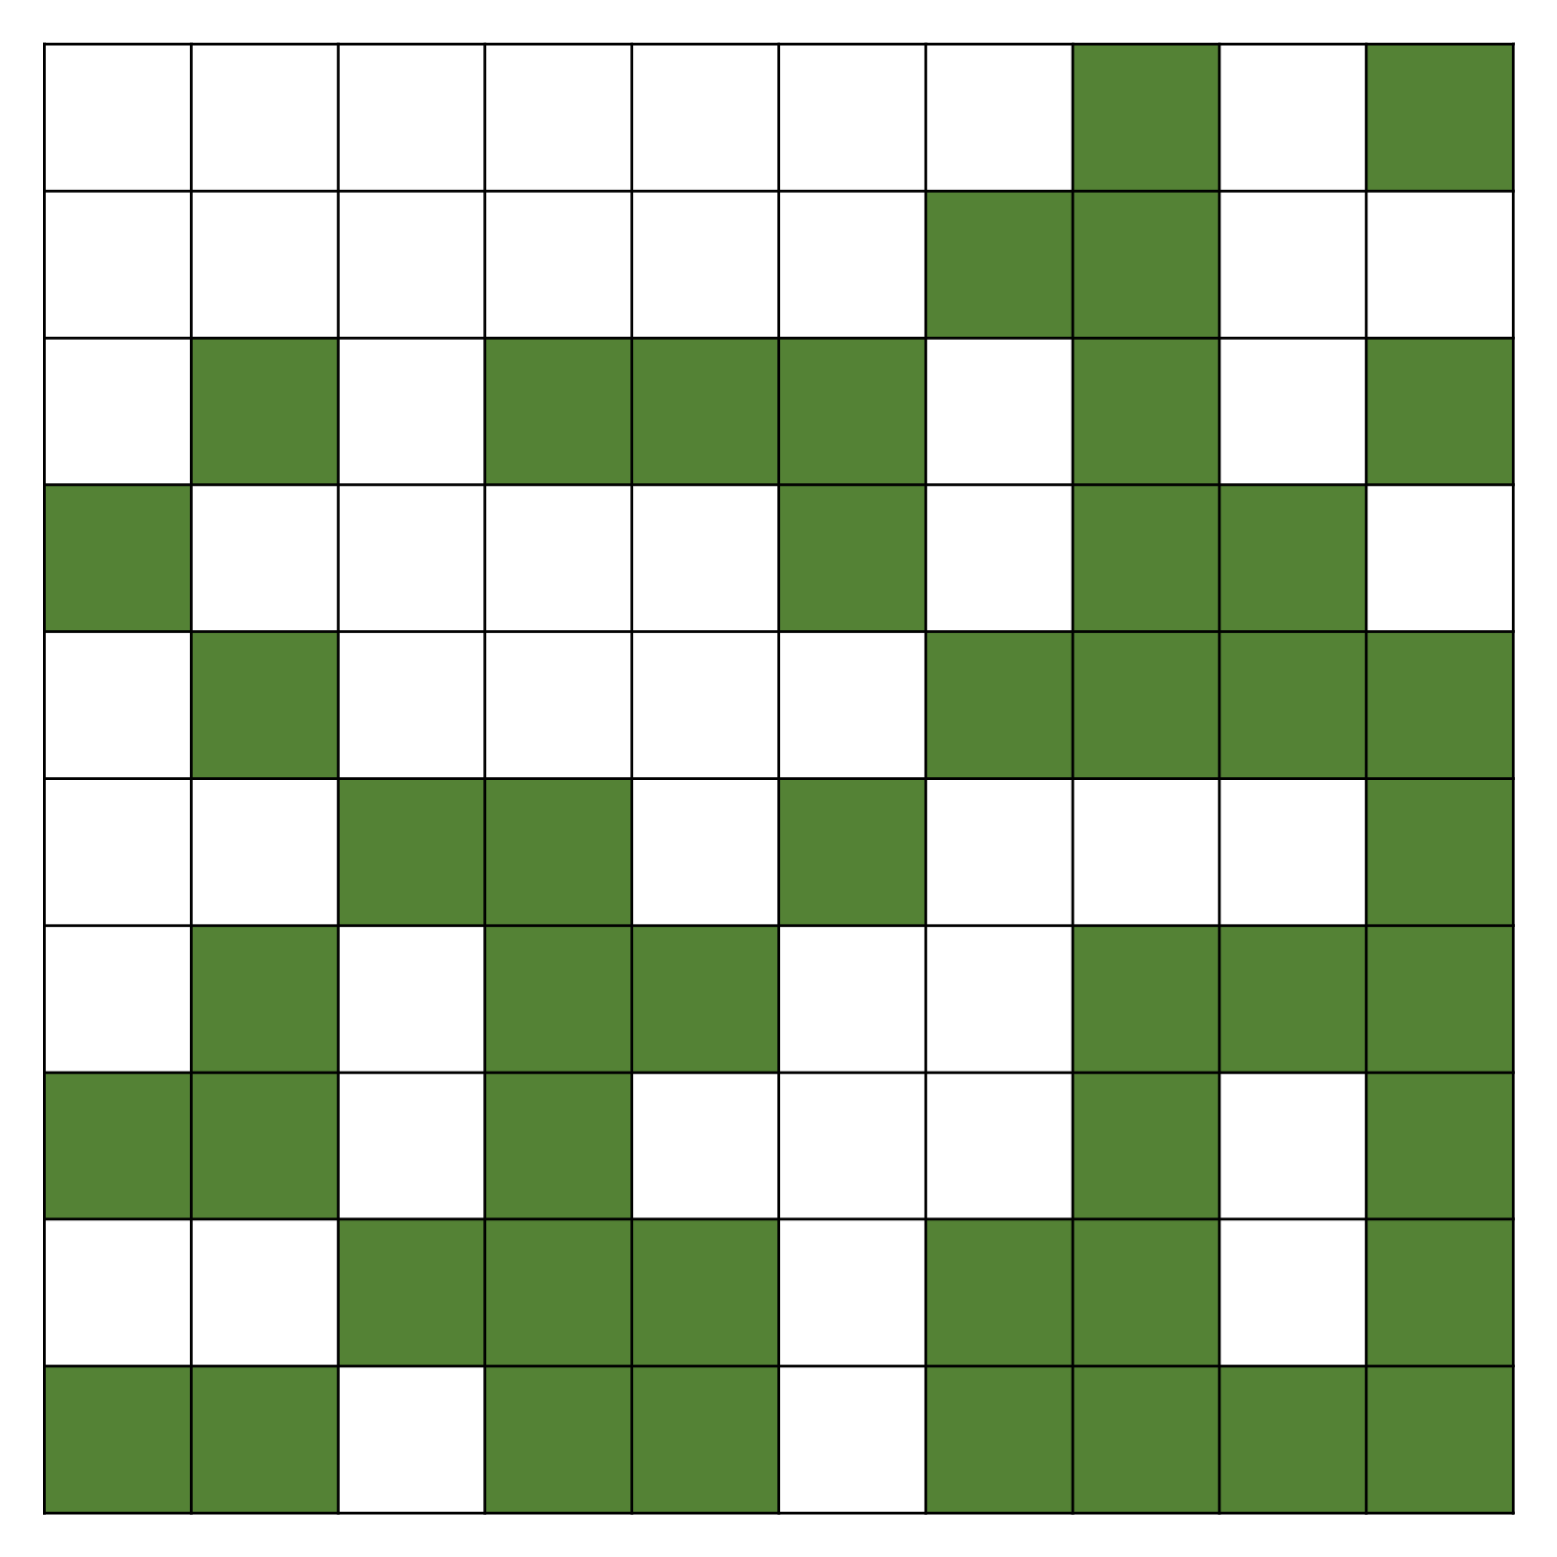
\includegraphics[width=0.4\linewidth]{firebreak/afterperc} 
    \caption{Graph after percolation ($p=1/2$)} 
    \label{fig:afterperc} 
    \vspace{4ex}
  \end{subfigure} 
  \begin{subfigure}{0.4\linewidth}
    \centering
    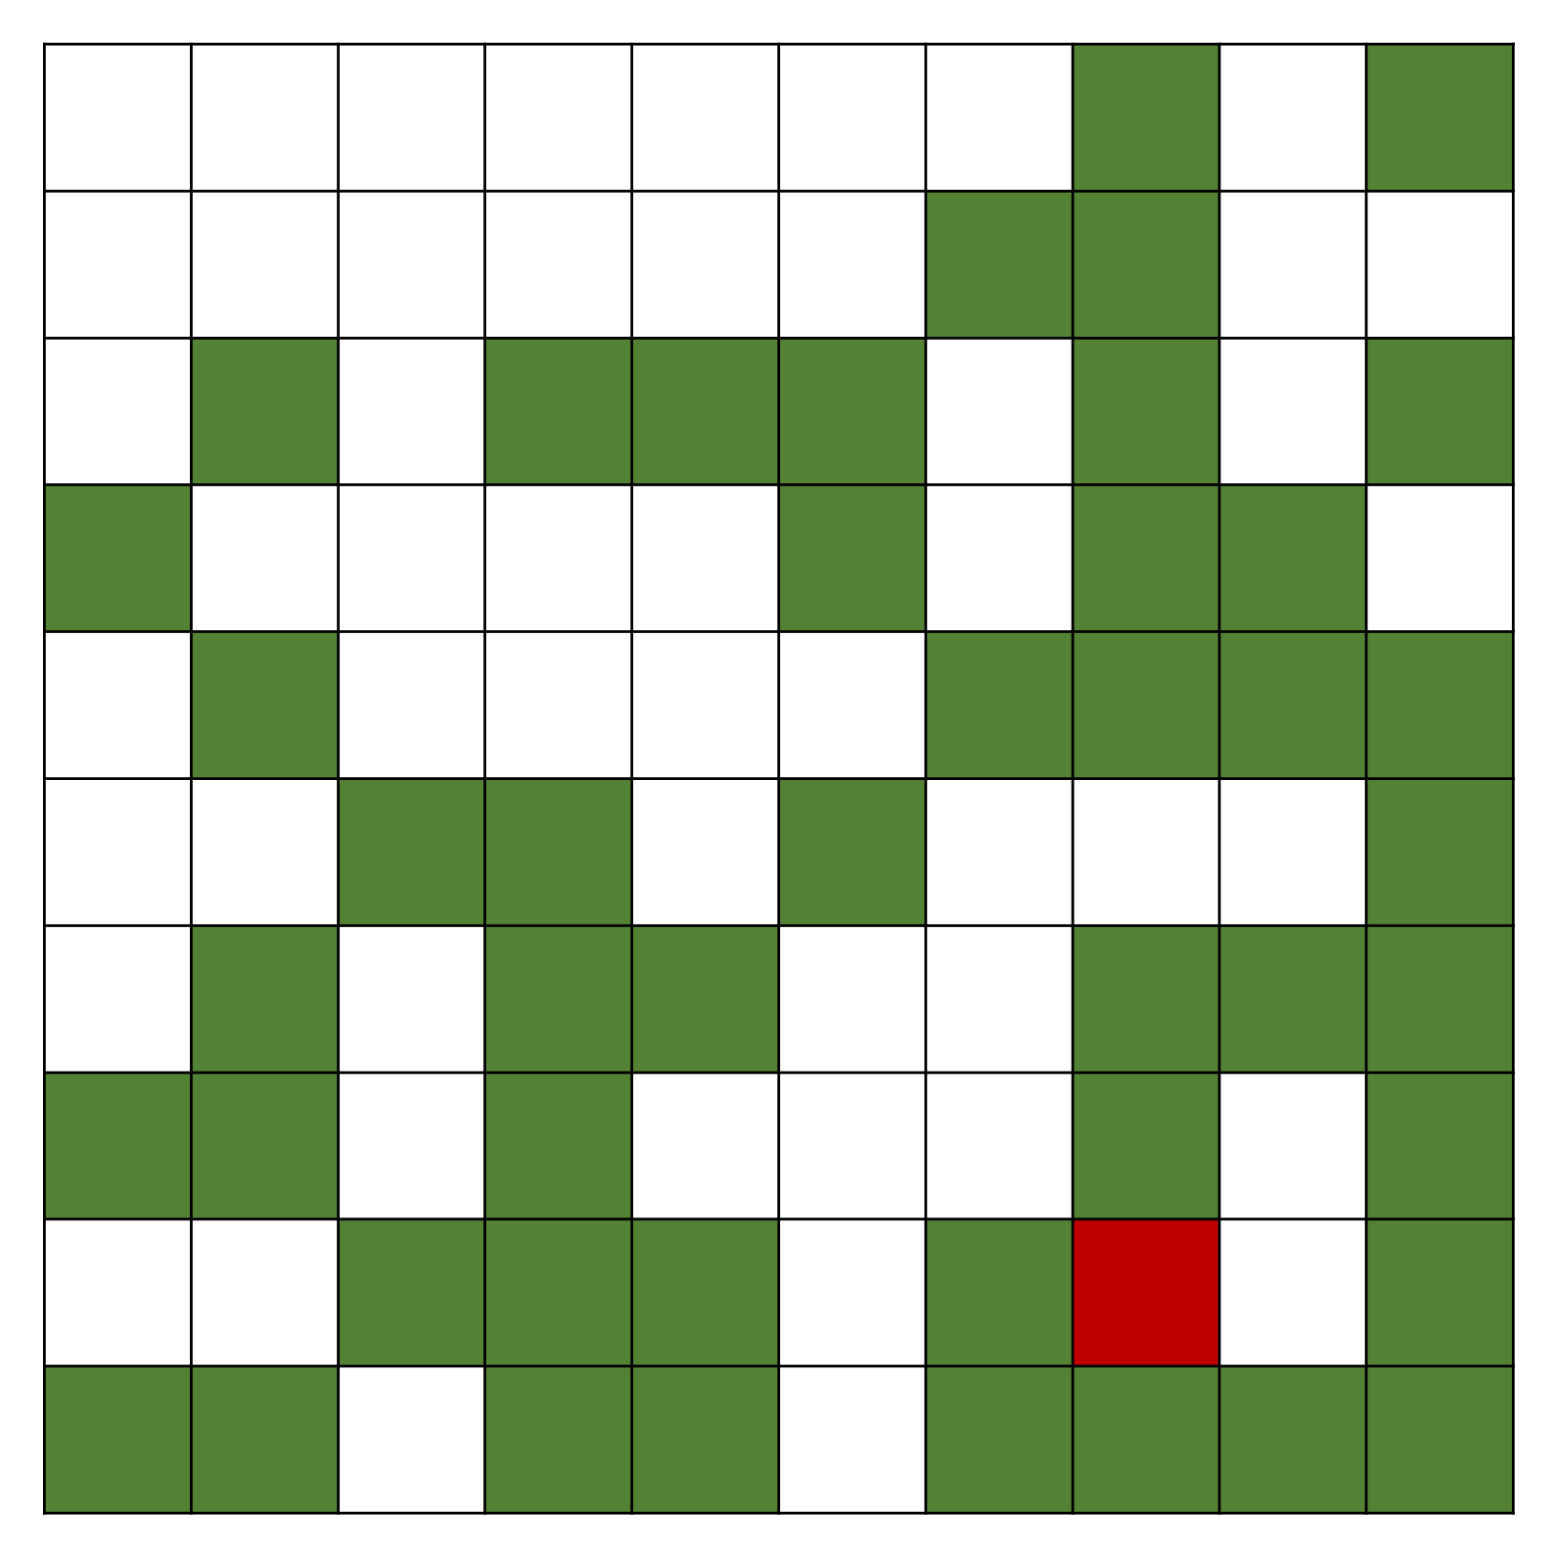
\includegraphics[width=0.4\linewidth]{firebreak/outbreak} 
    \caption{Initial outbreak ($t=0$)} 
    \label{fig:outbreak} 
  \end{subfigure}%%
  \begin{subfigure}{0.4\linewidth}
    \centering
    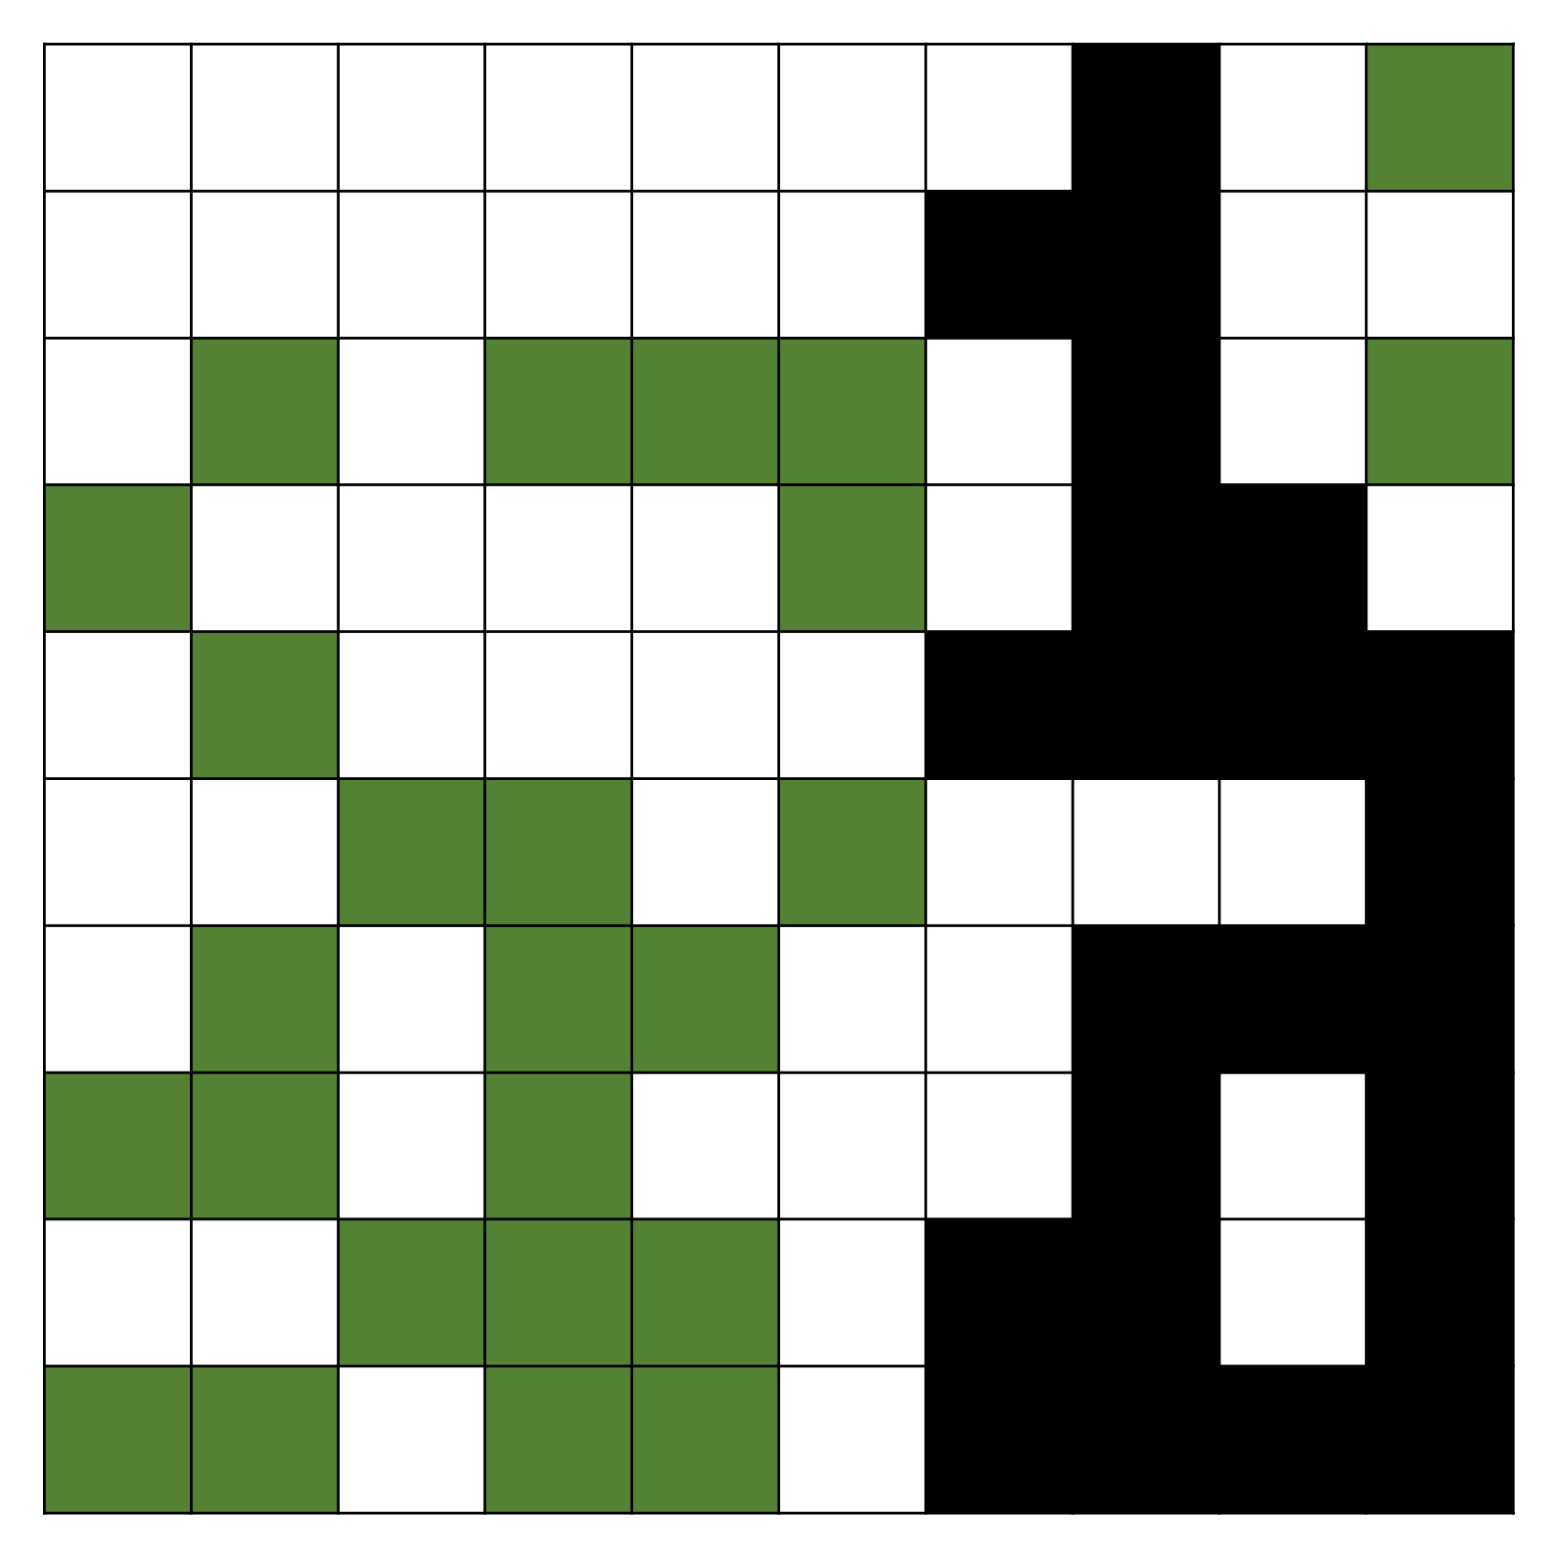
\includegraphics[width=0.4\linewidth]{firebreak/afteroutbreak} 
    \caption{End of outbreak ($t=12$)} 
    \label{fig:end} 
  \end{subfigure} 
  \caption{Outbreak of fire on a percolated graph}
  \label{fig:percolated_graph} 
\end{figure}

To illustrate this idea, we will consider a similar (perhaps precursor) to {\scshape Firefighter}, called The Firebreak Problem or simply {\scshape Firebreak}. Rather than have a firefighter reactively combatting the fire on each turn, we begin with an allocated amount of funding with which to mitigate the expected damage of the fire, and spend all of that before the fire begins. Generally, this means we have a number of edges to remove (trees to cut down or place a barrier in between) before the fire begins. Figure \ref{fig:percolated_graph} depicts the use of percolation on a graph to model a forest fire. We can see that the model would have little utility if we began the outbreak on the graph in \ref{fig:original} (all of the graph would be burnt), but percolation has made this a more instructive and realistic model in figure \ref{fig:afterperc}. We can see where the fire has spread in \ref{fig:end}, and we can see where - if we had a finite amount of resources - we must focus our efforts and funding in introducing a firebreak.\\

\begin{figure}[ht] 
  \begin{subfigure}{0.4\linewidth}
    \centering
    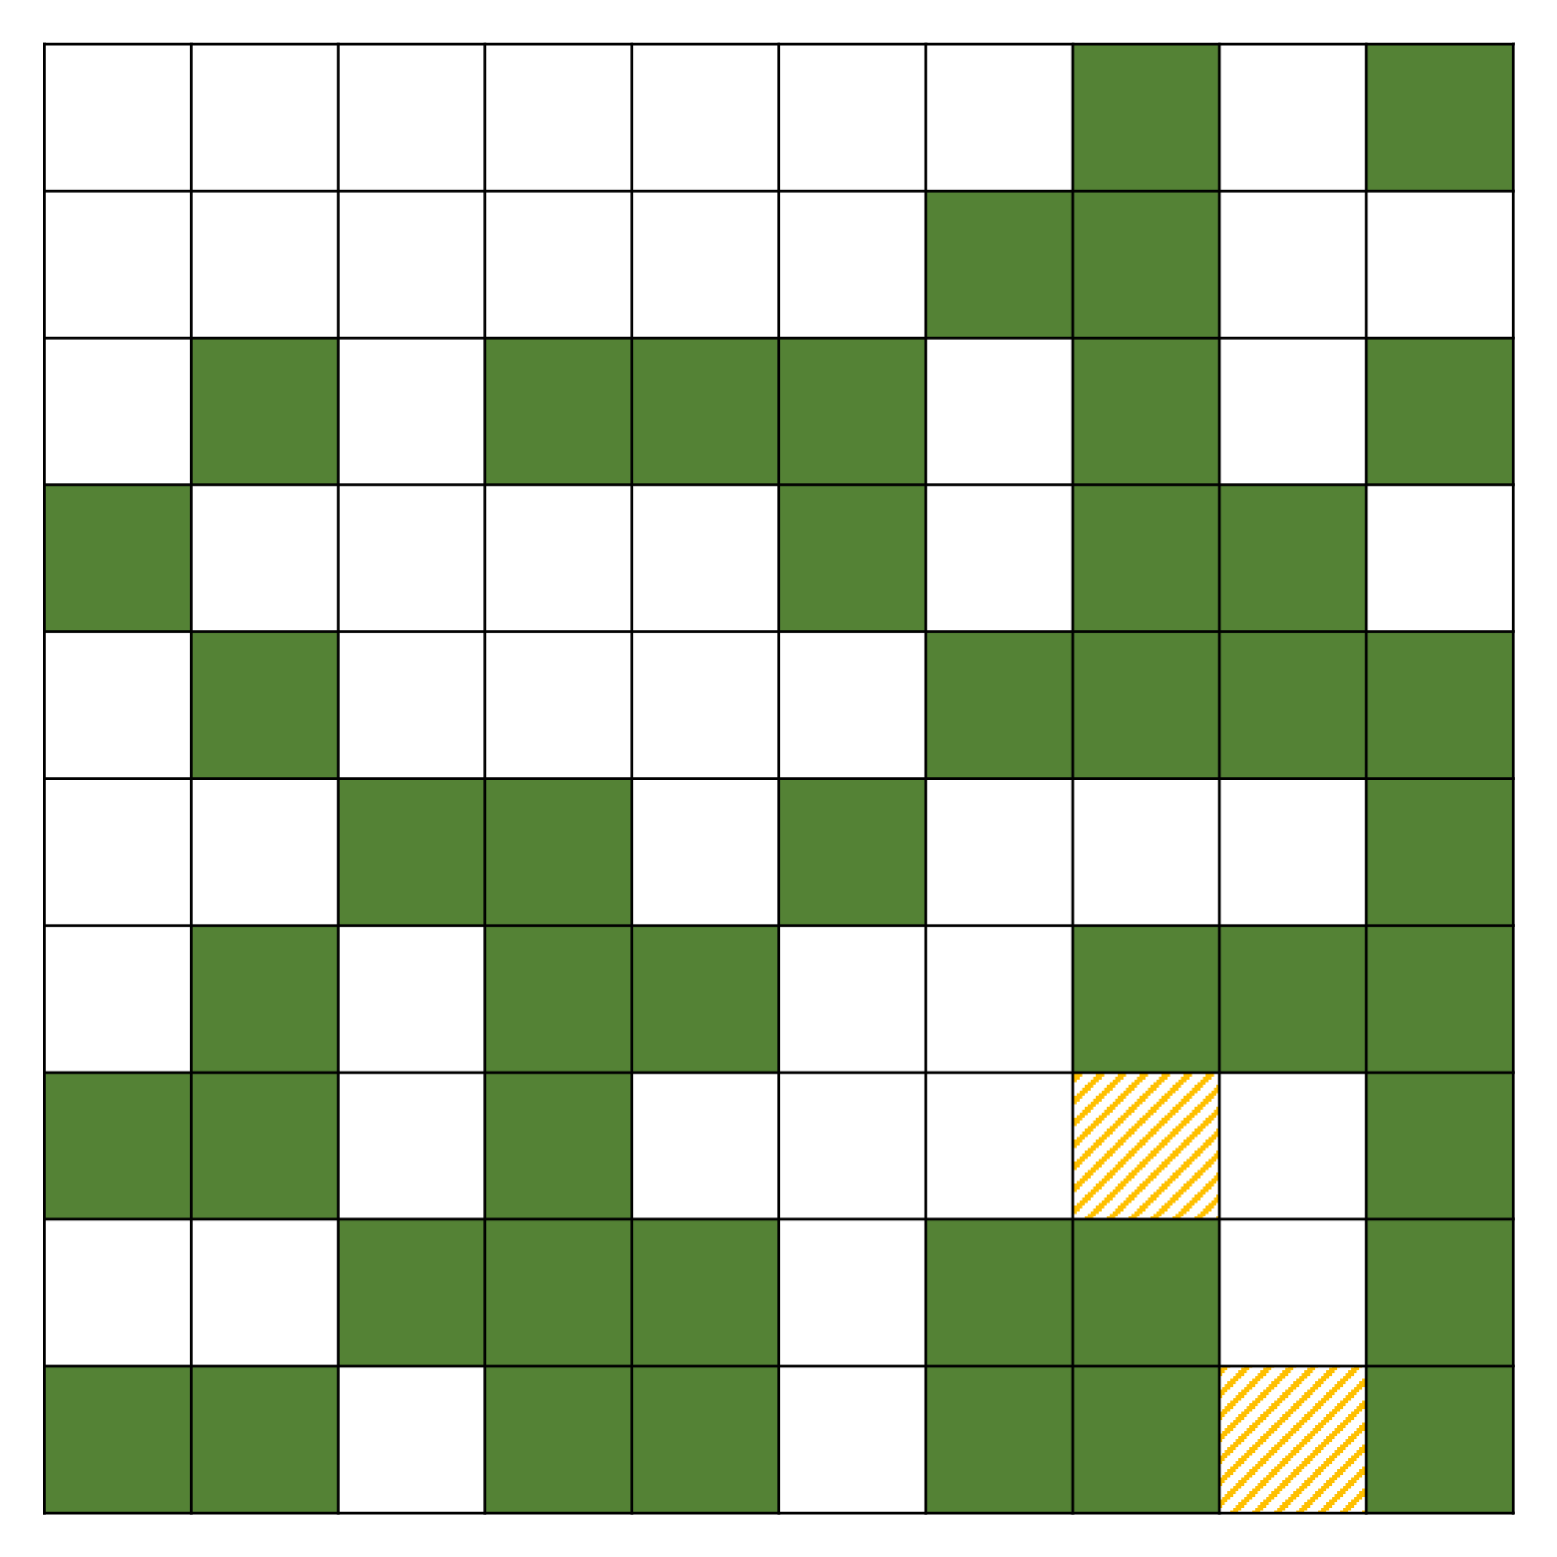
\includegraphics[width=0.4\linewidth]{firebreak/defended/defended} 
    \caption{Position of Firebreak (in yellow)} 
    \label{fig:defended} 
    %\vspace{4ex}
  \end{subfigure}%% 
  \begin{subfigure}{0.4\linewidth}
    \centering
    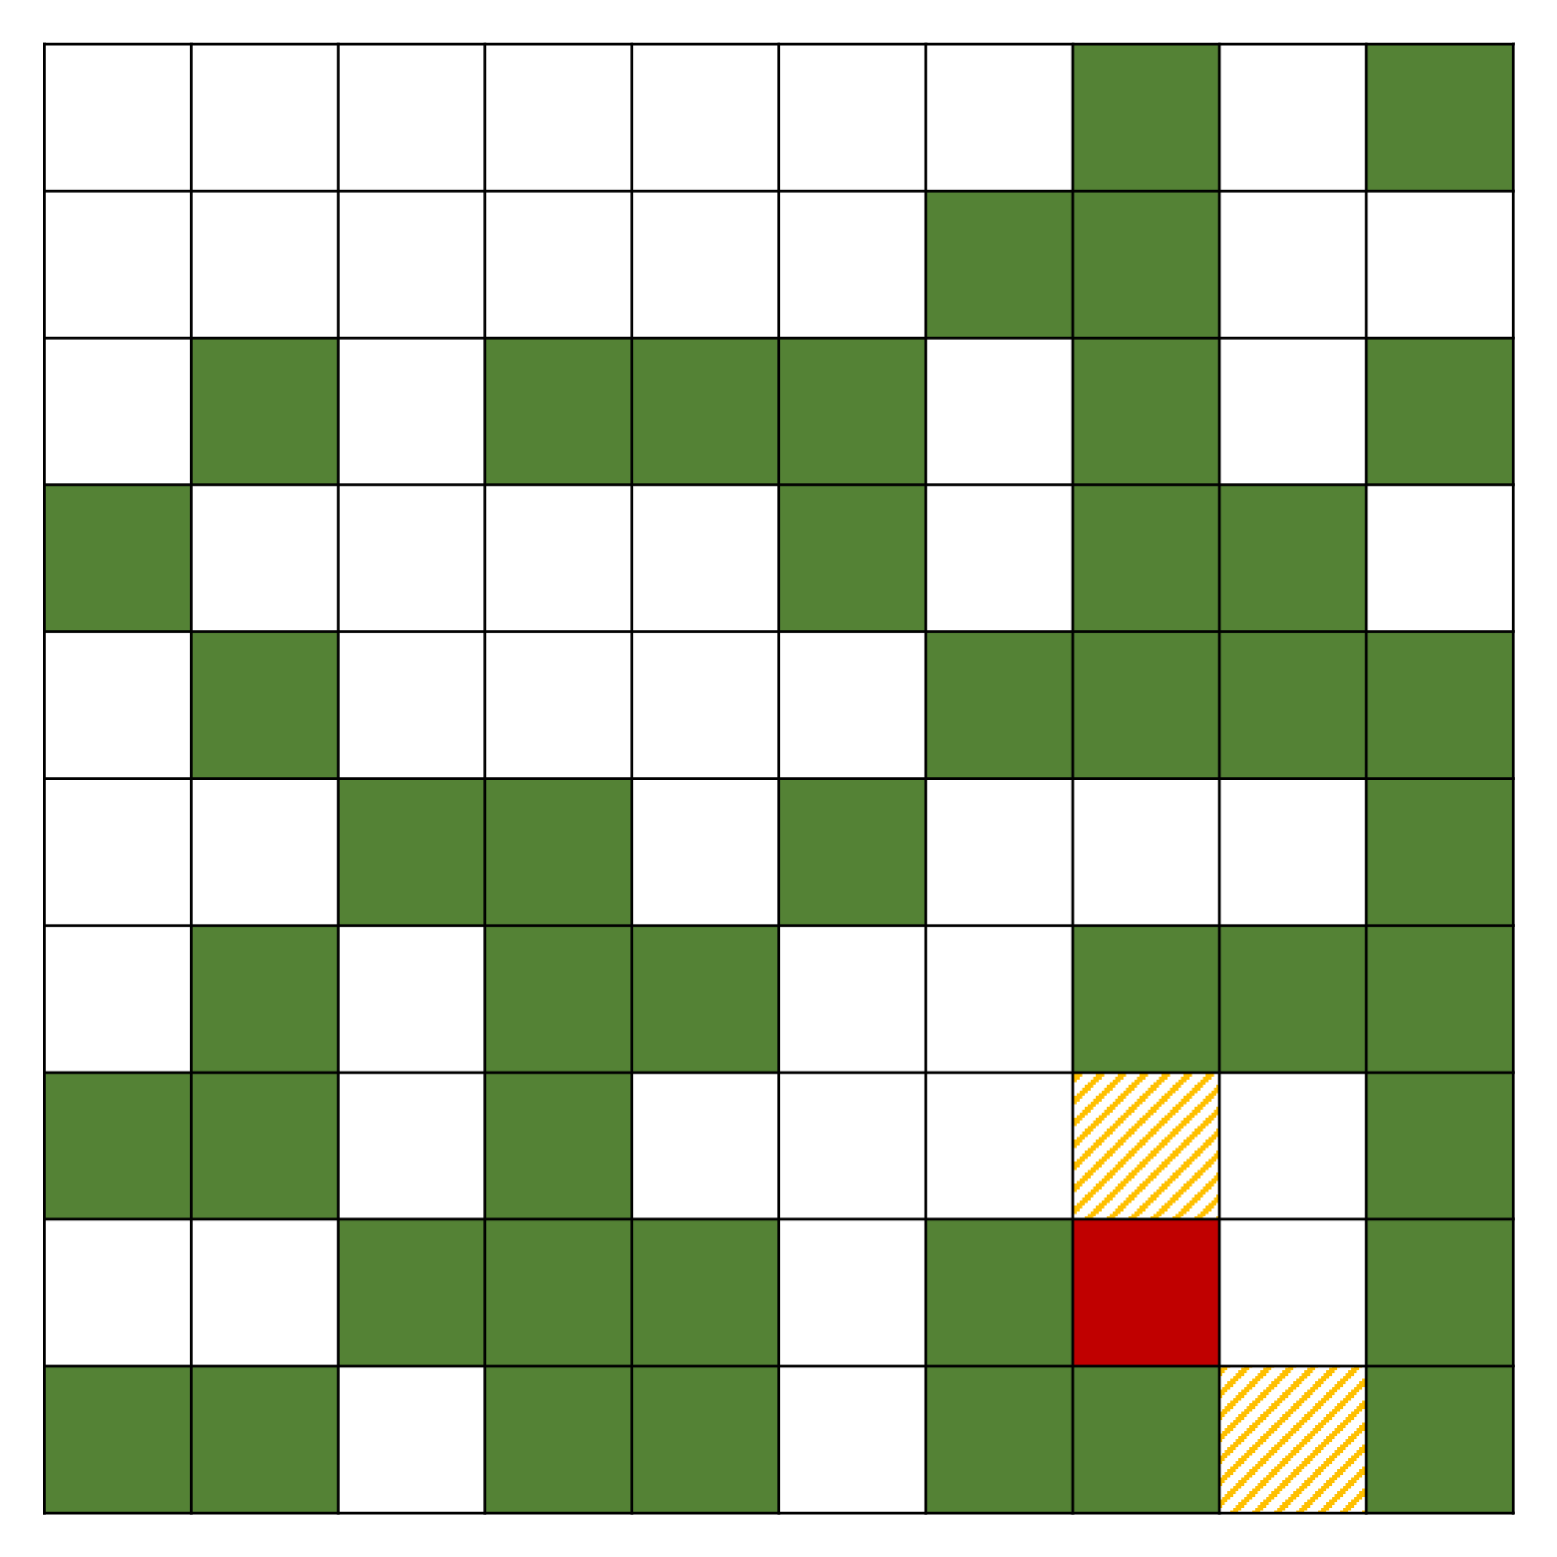
\includegraphics[width=0.4\linewidth]{firebreak/defended/outbreak} 
    \caption{Fire onset with firebreak ($t=0$)} 
    \label{fig:afterperc_break} 
    %\vspace{4ex}
  \end{subfigure}\\[1ex] 
  \begin{subfigure}{0.4\linewidth}
    \centering
    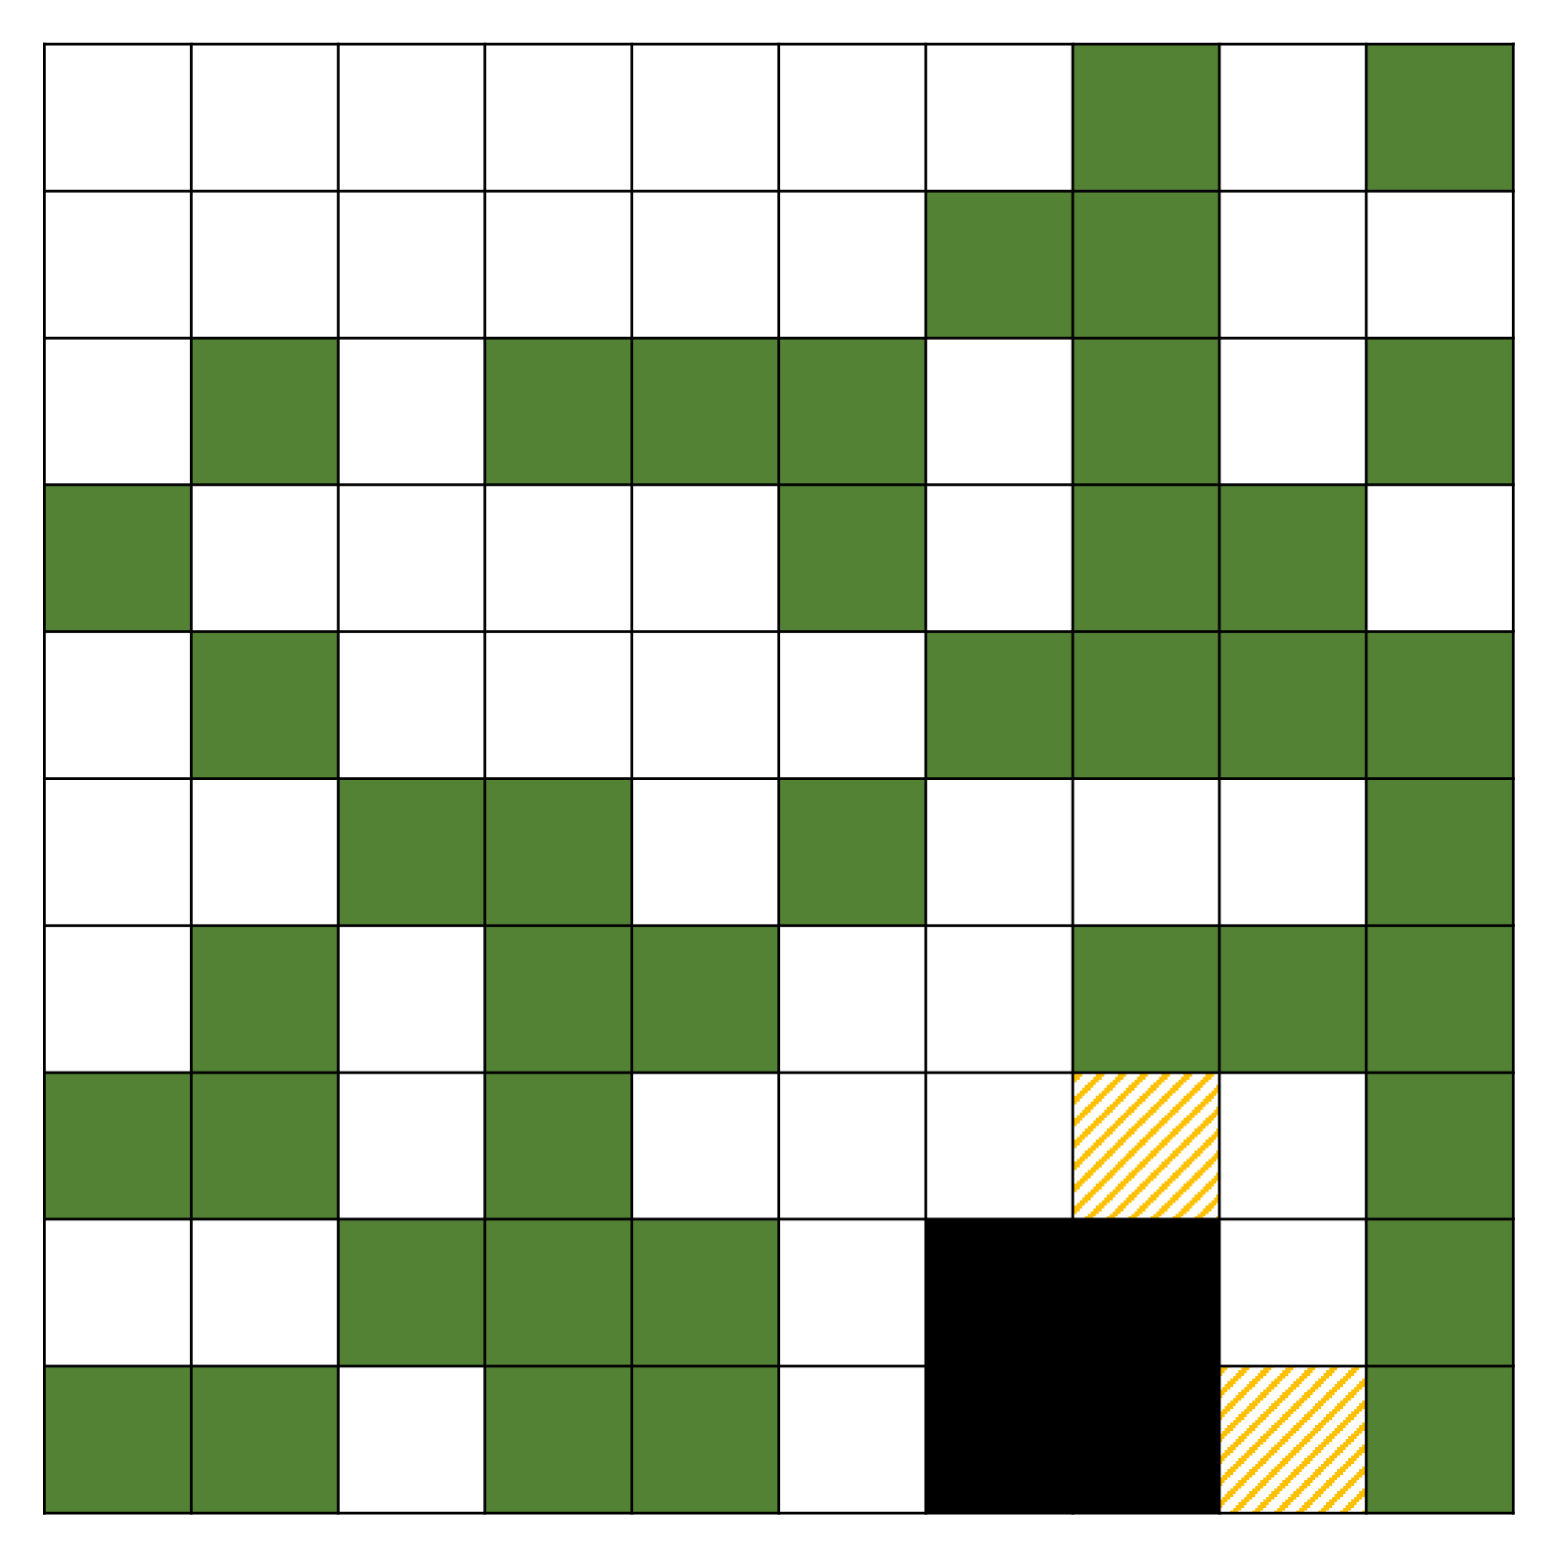
\includegraphics[width=0.4\linewidth]{firebreak/defended/end} 
    \caption{End of outbreak ($t=3$)} 
    \label{fig:end_defended} 
  \end{subfigure} 
  \caption{Outbreak of fire on a defended percolated graph}
  \label{fig:percolated_defended} 
\end{figure}

If, for instance, we could only remove two vertices as a firebreak, we ought to make those three the ones shown in yellow in figure \ref{fig:percolated_defended}. This is an example of how percolating a graph for use in {\scshape Firefighter} (and indeed {\scshape Firebreak}) can assist in generating a more realistic and useful model for contagion. There is much interest in the regular graph examples, but our modelling contexts of interest call for a more sporadic graph density and so we, in future research, will try and prove conjectures regarding the minimum number of vertex defences required in {\scshape Firebreak} for percolated graphs of given percolation threshold and dimension (or infinite graphs) and analogous questions in {\scshape Firefighter}.

\appendix
\section{Percolation in Mathematica}
\label{apx:mathematica}
Below is some sample Mathematica code for producing a helpful tool to visualise percolation on a network and finding the percolation threshold and is based on a Mathematica Stack Exchange question \cite{mathematica17}.
\begin{verbatim}

* Create sample dataset *
points = RandomReal[10 {-1, 1}, {200, 2}];

ListPlot[pts, AspectRatio -> Automatic, 
 Epilog -> {Red, Point[pts[[63]]], Point[pts[[90]]]}]

* Define distance matrix between points *
dst = Outer[EuclideanDistance, pts, pts, 1]; // Timing

* Set of possible edges in graph, sorted by length *
edges = Subsets[Range@Length[pts], {2}];
edges = SortBy[edges, Extract[dst, #] &];

* Index furthest left and right vertices as start and end *
start = First@Ordering[pts[[All, 1]], 1];
end = First@Ordering[pts[[All, 1]], -1];

* Get minimal length edge that we need to include *
idx = Module[{f}, Do[Set @@ f /@ (edges[[i]]);
   If[f[start] === f[end], Return[i]], {i, Length[edges]}]]

Extract[dst, edges[[idx]]]

* Manipulate to add edges one by one in increasing
   length until we have percolation threshold *
Manipulate[
 HighlightGraph[
  Graph[Range@Length@pts, UndirectedEdge @@@ Take[edges, i], 
   VertexCoordinates -> pts], {start, end}], {i, 1, idx, 1}]

\end{verbatim}

%%%%%%%%%%%%%%%%%%%%%%%%%%%%%%%%%%%%%%%%%%%%%%%%%%

\bibliographystyle{siam}
\bibliography{bibliography.bib}
%\nocite{*}

\Addresses

\end{document}  
